    %%%%%%%%%%%%%%%%%%%%%%%%%%%%%%%%%%%%%%%%
    %%  Slide 1: <BACKUP>  %%
    %%%%%%%%%%%%%%%%%%%%%%%%%%%%%%%%%%%%%%%%
    \begin{frame}
        Backup        
    \end{frame} 



    %%%%%%%%%%%%%%%%%%%%%%%%%%%%%%%%%%%%
    %% Slide 3: <> %%
    %%%%%%%%%%%%%%%%%%%%%%%%%%%%%%%%%%%%
    \begin{frame}
        \frametitle{Test on beam: preliminary results}
        \begin{itemize}
            \item With \textbf{both} the collimators, DPP=\SI{0.07}{Gy}, t$_p$=\SI{4}{\us}, PRF=\SI{1}{Hz}
        \end{itemize}
        \medskip
        \begin{figure}
            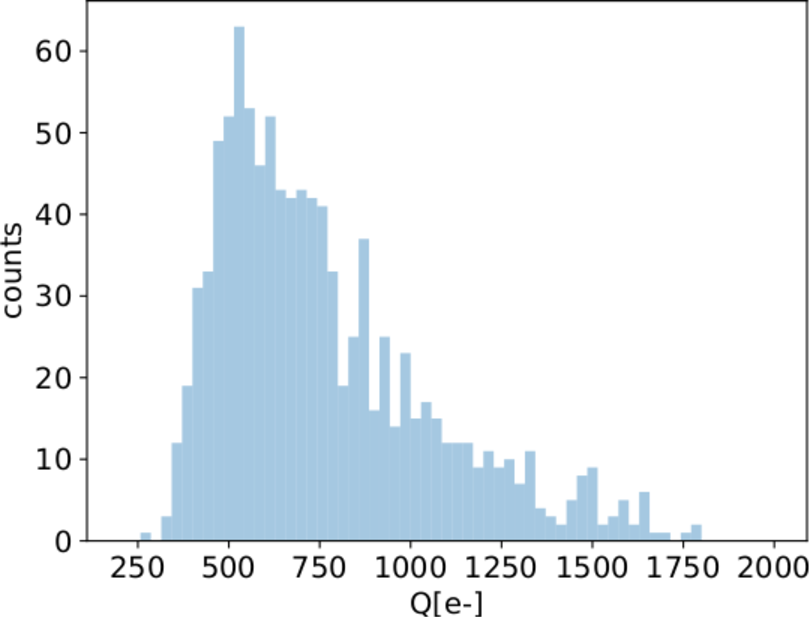
\includegraphics[width=0.49\linewidth]{figures/test_beam/Q1_17_11.pdf}
            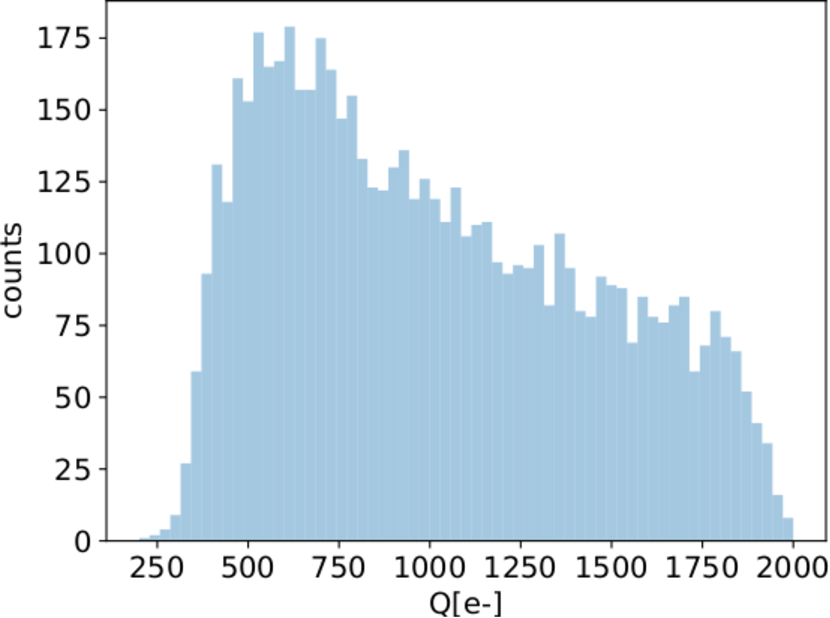
\includegraphics[width=.49\linewidth]{figures/test_beam/Q2_17_11.pdf}
        \end{figure}
        \begin{itemize}
            \item the collimators do not shield the detectors by all particles
            \item probably photons are produced by electrons in Al collimators
            \item for each accelerator pulse, 2 readout "cycle"  
        \end{itemize}
    \end{frame} 
    
    %%%%%%%%%%%%%%%%%%%%%%%%%%%%%%%%%%%%
    % Slide 3: <> %%
    %%%%%%%%%%%%%%%%%%%%%%%%%%%%%%%%%%%%
    \begin{frame}
        \frametitle{Test on beam: preliminary results}
        \begin{itemize}
            \item\textbf{Without} any collimator, DPP=\SI{0.04}{Gy}, t$_p$=\SI{4}{\us}, PRF=\SI{1}{Hz}
            \item MIP are expected to release \SI{2000}{\elementarycharge}$^-$, and because of rollorver are expected to be 300-400\si{\elementarycharge}$^-$
        \end{itemize}
        \medskip
        \begin{columns}
            \column{0.5\textwidth} 
                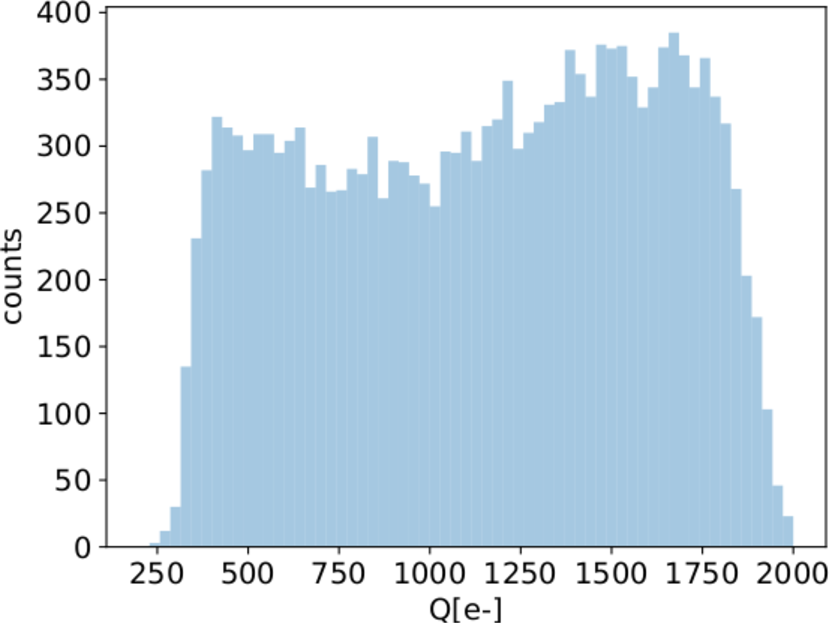
\includegraphics[width=1.1\linewidth]{figures/test_beam/Qe_17_32.pdf}
            \column{0.5\textwidth} 
                \begin{itemize}
                    \item ToT converted in charge
                    \item pixels turn on in N clock counts
                    \item after each pulse an induced signal on the whole matrix
                \end{itemize}
        \end{columns}   
        \medskip
        Need for a simulation to understand the data
    \end{frame}   